\documentclass{article}
\usepackage[utf8]{inputenc}
\usepackage{CJKutf8}
\usepackage{graphicx}
\usepackage{subfig}
\usepackage{float}

\usepackage{tikz}
\usepackage{xcolor}

% Custom colors
\definecolor{process0}{RGB}{144,202,249}  % Light blue
\definecolor{process1}{RGB}{165,214,167}  % Light green
\definecolor{process2}{RGB}{255,204,128}  % Light orange
\definecolor{process3}{RGB}{206,147,216}  % Light purple
\definecolor{halocell}{RGB}{239,154,154}  % Light red

\usepackage{dirtree}

% Layout
\usepackage[left=1.5in, right=1.5in, top=1in, bottom=1in]{geometry}

% Images
\graphicspath{{./images/}}
\usepackage{wrapfig}
\usepackage{tabularx}
\usepackage{multirow}
\usepackage{totalcount}
\usepackage{caption}
\captionsetup{skip=0pt} 




% Math
\usepackage{amsmath,amssymb,amsthm,enumitem,bm}

\DeclareMathOperator{\sech}{sech}
\DeclareMathOperator{\csch}{csch}
\DeclareMathOperator{\arcsec}{arcsec}
\DeclareMathOperator{\arccot}{arcCot}
\DeclareMathOperator{\arccsc}{arcCsc}
\DeclareMathOperator{\arccosh}{arcCosh}
\DeclareMathOperator{\arcsinh}{arcsinh}
\DeclareMathOperator{\arctanh}{arctanh}
\DeclareMathOperator{\arcsech}{arcsech}
\DeclareMathOperator{\arccsch}{arcCsch}
\DeclareMathOperator{\arccoth}{arcCoth}

\usepackage{listings}
\usepackage{parskip}
\setlength{\parindent}{0pt}

\begin{document}
% Title
\begin{center}
    \huge\textbf{M2: Lora Finetuning}
\end{center}



\begin{center}
    \Large Xueqing Xu (xx823)
    
    Department of Physics, University of Cambridge
    
    April 7, 2025
\end{center}

\section*{Introduction}
This coursework explores the application of Low-Rank Adaptation (LoRA) to fine-tune the Qwen2.5-Instruct Large Language Model (LLM) for forecasting predator-prey population dynamics. Building on the observation that LLMs can function as time series forecasters without explicit training\cite{gruver2023large}, we investigate how targeted fine-tuning can enhance their forecasting capabilities while maintaining efficiency.

LoRA represents a parameter-efficient fine-tuning technique that dramatically reduces the number of trainable parameters by injecting small, trainable low-rank matrices into existing model weights without modifying the original parameters. This approach is particularly valuable when working with large models under computational constraints.

The target application is forecasting the Lotka-Volterra predator-prey system, a classic ecological model that describes the dynamic interaction between two species. This system exhibits oscillatory behavior that presents a challenging forecasting task requiring understanding of non-linear dynamics and the ability to model complex interdependencies.
\section*{Methodology}
\subsection*{Qwen2.5-Instruct model architecture}
The Qwen2.5-0.5B-Instruct model implements a decoder-only transformer architecture with 494 million parameters (Table \ref{tab:qwen25-overview}). With a hidden dimension of 896 across 24 transformer layers, the model balances depth and computational efficiency.

A key architectural feature is Grouped Query Attention (GQA), which employs 14 query heads but only 2 key-value heads—a 7:1 ratio that substantially reduces memory usage during inference while maintaining attention capabilities. For normalization, Qwen2.5 uses RMSNorm with $\epsilon = 10^{-6}$, which offers better training stability than traditional LayerNorm.
% Qwen2.5-0.5B-Instruct Model Overview Table
\begin{table}[ht]
\centering
\begin{tabular}{ll}
\hline
\textbf{Parameter} & \textbf{Value} \\
\hline
Model Type & Decoder-only Transformer \\
Parameters & 0.5 Billion \\
Hidden Size & 896 \\
Attention Heads & 14 \\
Head Dimension & 64 \\
Number of Layers & 24 \\
Intermediate Size (MLP) & 4864 \\
Vocabulary Size & 151,936 \\
\hline
\multicolumn{2}{l}{\textbf{Layer Structure (Repeated 24 times):}} \\
\hline
Pre-Attention & RMSNorm \\
Attention & Multi-head attention with RoPE \\
& \quad - Q, K, V projections \\
& \quad - Rotary Position Embeddings \\
Post-Attention & Residual connection \\
Pre-MLP & RMSNorm \\
MLP & Gate and Up projections \\
& SwiGLU activation \\
& Down projection \\
Post-MLP & Residual connection \\
\hline
\textbf{Final Output} & RMSNorm + Linear (LM head) \\
\hline
\end{tabular}
\caption{Qwen2.5-0.5B Model Architecture}
\label{tab:qwen25-overview} 
\end{table}
The model implements Rotary Position Embeddings (RoPE) with a base frequency of 1,000,000.0 to encode relative positions effectively, supporting its 32K token context window. As shown in Table \ref{tab:qwen25-overview}, each layer consists of self-attention and feed-forward blocks, both with pre-normalization and residual connections. The feed-forward network uses SwiGLU activation and an intermediate dimension of 4864 (approximately 5.4× the hidden size).

\subsubsection*{Key Components with Mathematical Definitions}

\textbf{RMSNorm (Root Mean Square Normalization):} Unlike traditional LayerNorm, RMSNorm eliminates mean-centering and focuses only on variance normalization:

\begin{equation}
\text{RMSNorm}(x) = \frac{x}{\sqrt{\frac{1}{n}\sum_{i=1}^{n}x_i^2 + \epsilon}} \cdot \gamma
\end{equation}

\noindent where $\epsilon = 10^{-6}$ is a small constant for numerical stability, and $\gamma$ represents trainable scale parameters.

\textbf{SiLU (Swish) Activation:} The SiLU activation function used in the feed-forward networks is defined as:
\begin{equation}
\text{SiLU}(x) = x \cdot \sigma(x) = \frac{x}{1 + e^{-x}}
\end{equation}

\noindent where $\sigma(x)$ is the sigmoid function. This activation combines properties of both ReLU and sigmoid functions.

\textbf{Rotary Position Embeddings (RoPE):} RoPE\cite{su2024roformer} encodes position information through rotation matrices in the complex plane:

\begin{equation}
\mathbf{q}_{m,i}^{\theta} = \begin{pmatrix} \cos(m\theta_i) & -\sin(m\theta_i) \\ \sin(m\theta_i) & \cos(m\theta_i) \end{pmatrix} \mathbf{q}_{m,i}
\end{equation}

\noindent where $\mathbf{q}_{m,i}$ represents query vector components, $m$ is the position index, and $\theta_i$ denotes frequencies constructed with base $\theta = 1,000,000.0$.

\textbf{SwiGLU Feed-Forward Network:} The FFN in each layer consists of three projections:

\begin{enumerate}
\item \textbf{Gate Projection:} $G(x) = W_g x$, where $W_g \in \mathbb{R}^{4864 \times 896}$
\item \textbf{Up Projection:} $U(x) = W_u x$, where $W_u \in \mathbb{R}^{4864 \times 896}$
\item \textbf{Down Projection:} $D(x) = W_d x$, where $W_d \in \mathbb{R}^{896 \times 4864}$
\end{enumerate}

The complete FFN operation is defined as:
\begin{equation}
\text{FFN}(x) = D(\text{SiLU}(G(x)) \odot U(x))
\end{equation}

\noindent where $\odot$ represents element-wise multiplication.

% Qwen2.5-0.5B-Instruct Vocabulary Details Table
\begin{table}[H]
\centering
\begin{tabular}{@{}ll@{}}
\hline
\textbf{Property} & \textbf{Value} \\
\hline
Vocabulary Size & 151,936 tokens \\
BOS Token ID & 151,643 \\
EOS Token ID & 151,645 \\
Word Embeddings & Tied with output layer \\
\hline
\end{tabular}
\caption{Qwen2.5-0.5B-Instruct Vocabulary Details}
\label{tab:qwen25-vocab}
\end{table}

The model implements these components with a vocabulary of 151,936 tokens and tied word embeddings between input and output layers (Table \ref{tab:qwen25-vocab}). This architecture is particularly suitable for parameter-efficient fine-tuning methods like LoRA, as we can target high-leverage components (query and value projections) while keeping most parameters frozen.
\subsection*{Lora Finetuning}
Low-Rank Adaptation (LoRA) \cite{hu2022lora} represents a parameter-efficient fine-tuning approach that substantially reduces the number of trainable parameters while maintaining model performance. The key innovation lies in decomposing weight updates into low-rank matrices instead of fine-tuning the entire weight matrices.

\subsubsection*{Mathematical Formulation}

In standard fine-tuning of a pre-trained model, the weight matrix $W_0 \in \mathbb{R}^{d \times k}$ is updated to $W = W_0 + \Delta W$ during training. LoRA parameterizes the update $\Delta W$ using two low-rank matrices:

\begin{equation}
W = W_0 + \Delta W = W_0 + BA
\end{equation}

where $B \in \mathbb{R}^{d \times r}$ and $A \in \mathbb{R}^{r \times k}$ with rank $r \ll \min(d,k)$. During the forward pass, for input $x$, the output is computed as:


\begin{equation}
    h = W_0x + \Delta Wx = W_0x + BAx
    \end{equation}
    
    The weight update is typically scaled during training by $\alpha/r$, where $\alpha$ is a constant hyperparameter:
    
    \begin{equation}
    h = W_0x + \frac{\alpha}{r}BAx
    \end{equation}
    
    \subsubsection*{Application to Qwen2.5}
    
    For the Qwen2.5-0.5B-Instruct model, we apply LoRA specifically to the query and value projection matrices in the multi-head attention mechanism. These matrices are chosen because:
    
    \begin{itemize}
        \item Query projections ($W_q \in \mathbb{R}^{896 \times 896}$) directly influence the model's ability to focus on relevant context
        \item Value projections ($W_v \in \mathbb{R}^{896 \times 128}$) affect how the model represents information for aggregation
        \item Modifying these components provides substantial adaptation power while minimizing parameter count
    \end{itemize}
The LoRA matrices are injected into the model architecture, allowing for efficient adaptation without altering the original weights. The choice of low-rank matrices enables us to maintain a small number of trainable parameters while still achieving significant performance improvements.
    \subsubsection*{Training Dynamics}

During training, only the LoRA parameters ($A$ and $B$) are updated while $W_0$ remains frozen. This approach offers several advantages:

\begin{itemize}
    \item \textbf{Memory efficiency}: Only the gradients for LoRA parameters need to be stored
    \item \textbf{Composability}: Multiple task-specific LoRA modules can be trained and swapped without changing the base model
    \item \textbf{Preservation of general knowledge}: The original pre-trained weights remain intact
\end{itemize}

In our implementation, we utilized the transposed form of the LoRA matrices during the forward pass, computing the update as \texttt{self.lora\_A.T @ self.lora\_B.T}. This approach is mathematically equivalent to the original formulation but offers implementation advantages within the PyTorch framework, particularly for gradient computation efficiency.

Additionally, we deviated from the standard LoRA approach by making the language model head trainable as well. This decision was motivated by the need for adaptation specifically at the vocabulary distribution level, which is crucial for accurate numerical predictions. The LM head contains $896 \times 151,936 = 136,134,656$ parameters, significantly increasing our trainable parameter count, but targeting this layer directly improves the model's ability to produce precise numerical outputs in text form.

The total trainable parameter count thus becomes:
\begin{align}
\text{LoRA parameters} + \text{LM head parameters} &= 344,064 + 136,134,656\\
&= 136,478,720
\end{align}

This still represents a significant reduction (approximately 72.4\%) compared to full fine-tuning of all 494 million parameters.
\subsection*{Predator-Prey Dynamics}

The Lotka-Volterra model represents a classic mathematical framework for studying predator-prey interactions in ecological systems. It describes the oscillatory dynamics between two populations: a prey species ($x$) that has abundant food and can reproduce exponentially, and a predator species ($y$) that relies on consuming the prey for survival.

\subsubsection*{Mathematical Model}

The standard Lotka-Volterra equations are defined as:

\begin{align}
\frac{dx}{dt} &= \alpha x - \beta xy \\
\frac{dy}{dt} &= \delta xy - \gamma y
\end{align}

In these equations, $x(t)$ and $y(t)$ represent the prey and predator populations at time $t$, respectively. The parameter $\alpha$ denotes the prey's natural growth rate, while $\beta$ represents the predation rate, capturing the effect of predators on prey population decline. For predators, $\delta$ quantifies their reproduction rate per prey consumed, and $\gamma$ represents their natural mortality rate in the absence of prey.

\subsubsection*{Data Analysis}

Our exploratory analysis of the Lotka-Volterra dataset revealed important statistical properties across 1,000 trajectories. Each trajectory contained 100 time points with consistent sampling intervals. Data quality checks verified the absence of duplicates and negative values. 

Using K-means clustering on trajectory features (including period, amplitude, and phase relationships), we identified four distinct dynamic patterns in the dataset as displayed in Figure \ref{fig:clusters}:

\begin{itemize}
\item \textbf{Classic oscillatory dynamics (14.6\%)}: Characterized by sustained oscillations with relatively balanced prey and predator populations, showing clear cyclic interactions.
\item \textbf{Prey-dominant systems (69.3\%)}: Systems where prey populations maintain higher relative values with predator populations showing dampened oscillations.
\item \textbf{Equilibrium systems (14.9\%)}: Trajectories that stabilize after initial oscillations, reaching a relatively steady state.
\item \textbf{Predator collapse systems (1.2\%)}: A small subset where predator populations drop dramatically, allowing prey populations to grow significantly without constraint.
\end{itemize}

\begin{figure}[H]
    \centering
    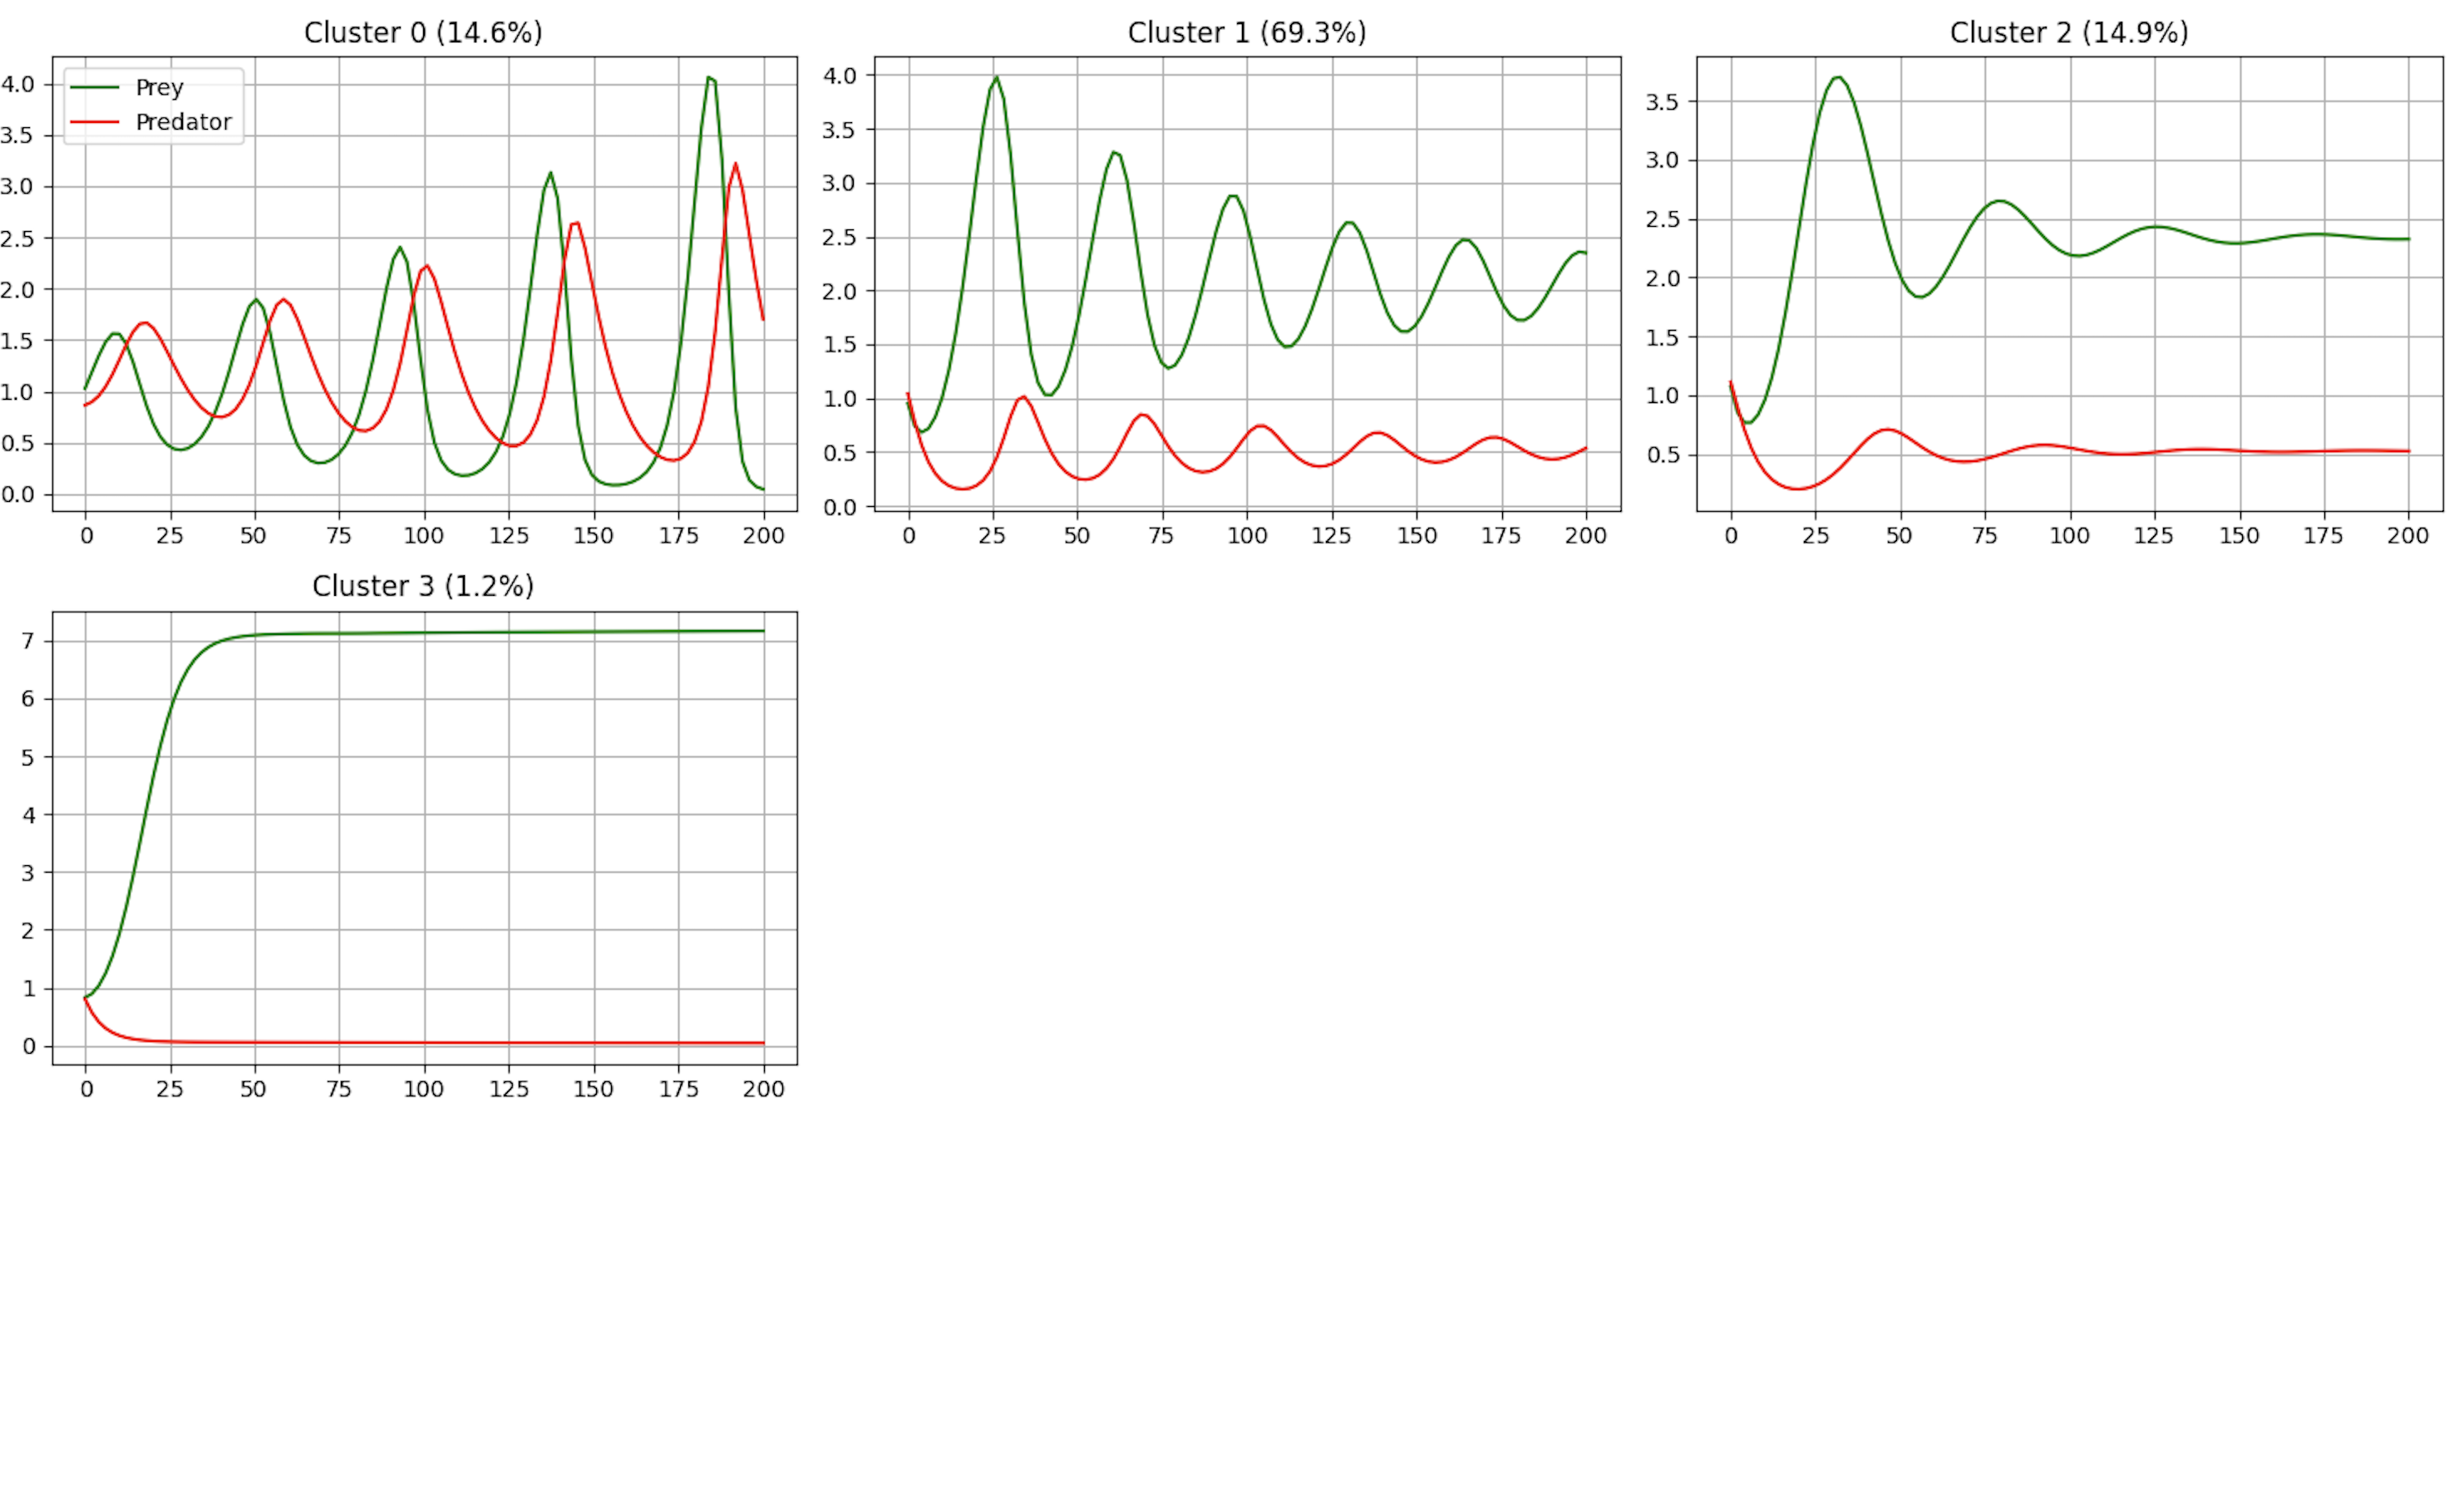
\includegraphics[width=0.8\textwidth]{cluster_representatives}
    \caption{\textbf{Cluster Analysis}. Four distinct clusters identified in the Lotka-Volterra dataset through K-means clustering, showing different regime types: classic oscillatory dynamics (14.6\%), prey-dominant systems (69.3\%), equilibrium systems (14.9\%), and predator collapse systems (1.2\%).}
    \label{fig:clusters}
\end{figure}

The clustering revealed that the majority of systems (69.3\%) fall into prey-dominant dynamics, suggesting parameter combinations that favor prey survival across much of the parameter space explored.

Figure \ref{fig:trajectories} showcases individual trajectories representing diverse dynamic behaviors within the dataset. These examples highlight the variability in amplitudes, frequencies, and phase relationships that our forecasting model must learn to predict accurately.

Through peak detection analysis, we calculated oscillation periods for both prey and predator populations, finding average periods of approximately 20-25 time units for prey and 20-30 time units for predators, as shown in Figure \ref{fig:periods}.

Further analysis of the phase relationships between prey and predator oscillations showed that predator peaks typically lag behind prey peaks by about 0.2 time units (20\% of the cycle period), as illustrated in Figure \ref{fig:periods}. This characteristic phase difference reflects the biological reality that predator populations grow in response to increasing prey availability, then decline as prey becomes scarce.

\begin{figure}[H]
    \centering
    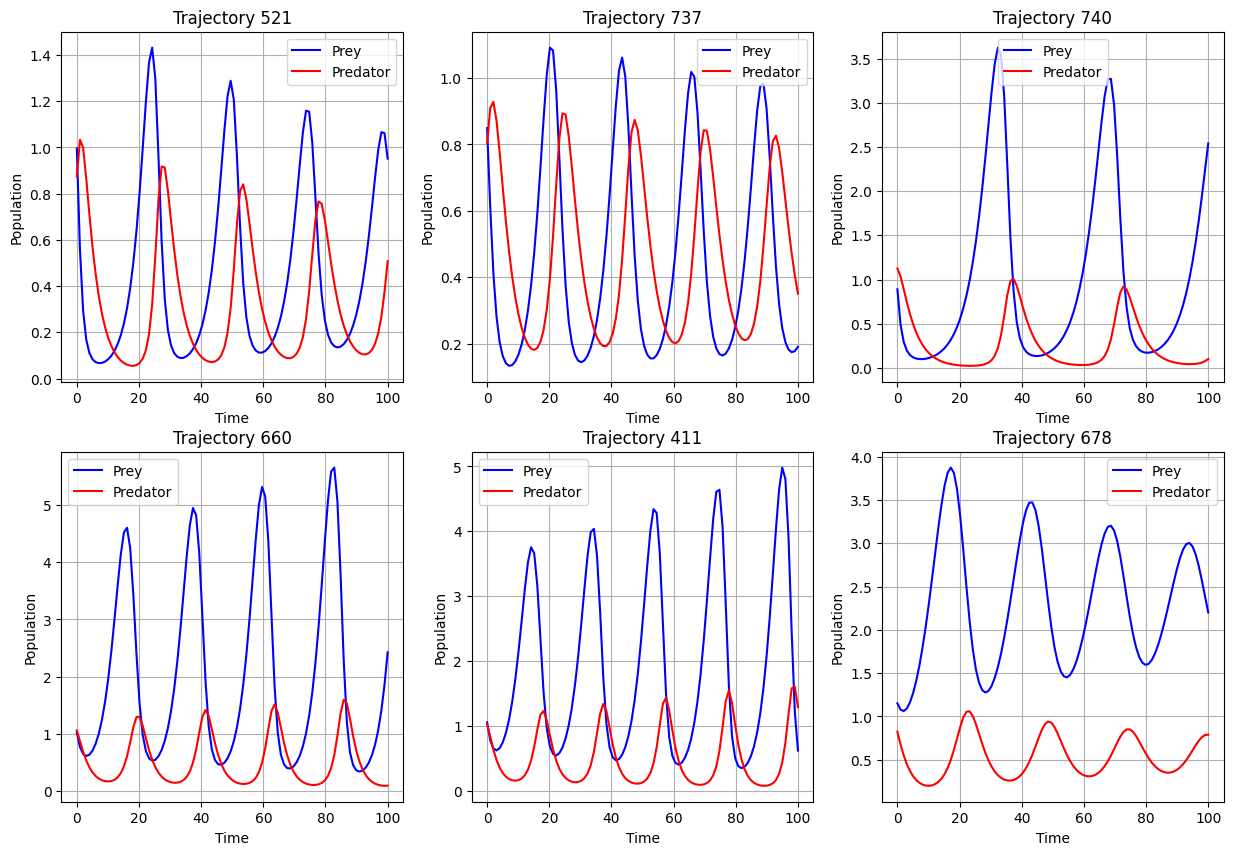
\includegraphics[width=0.8\textwidth]{sample}
    \caption{\textbf{Individual Trajectories}. Sample trajectories of prey and predator populations in the Lotka-Volterra dataset, illustrating the oscillatory dynamics characteristic of the model.}
    \label{fig:trajectories}
\end{figure}


\begin{figure} [H]
    \centering
    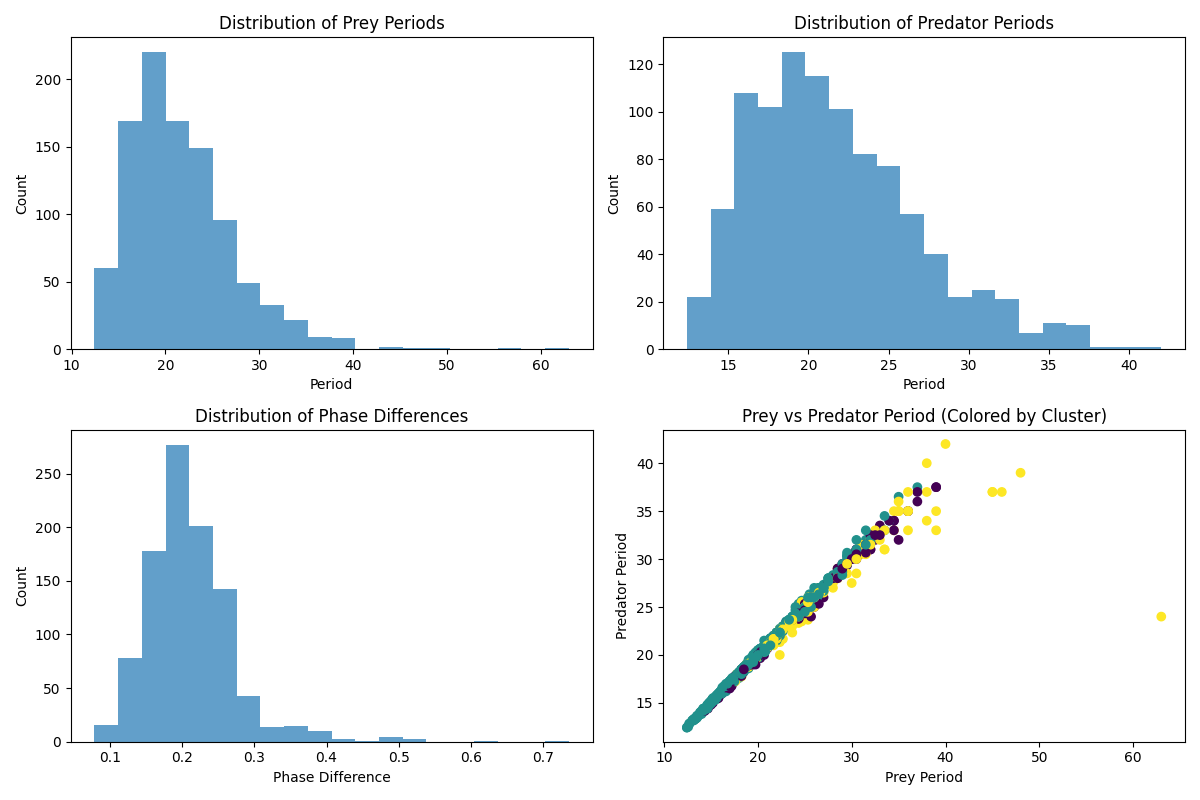
\includegraphics[width=0.8\textwidth]{period_distributions}
    \caption{\textbf{Statistical Distributions}. Distribution of oscillation periods for prey and predator populations in the Lotka-Volterra dataset, highlighting the variability in dynamics across different parameter regimes. }
    \label{fig:periods}
\end{figure}

Figure \ref{fig:average_trajectories} reveals typical system behavior with prey populations maintaining higher values (averaging $\approx$ 1.7 units) compared to predator populations (averaging $\approx$ 0.6 units) after initial transient dynamics.

\begin{figure} [H]
    \centering
    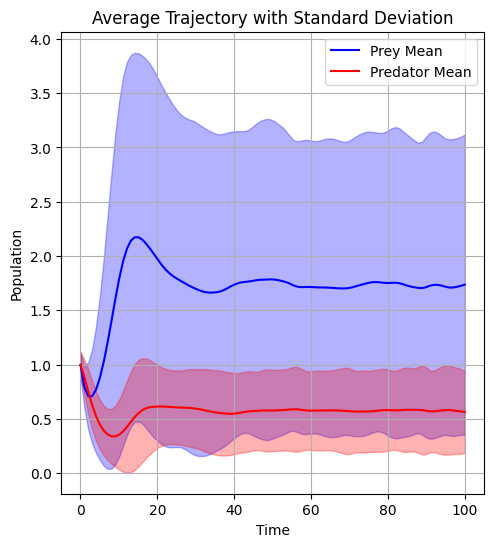
\includegraphics[width=0.5\textwidth]{overview_distribution}
    \caption{\textbf{Average Trajectories}. Average population trajectories with uncertainty: Mean prey (blue) and predator (red) population trajectories over time with shaded regions representing standard deviation.}
    \label{fig:average_trajectories}
\end{figure}

\begin{figure} [H]
    \centering
    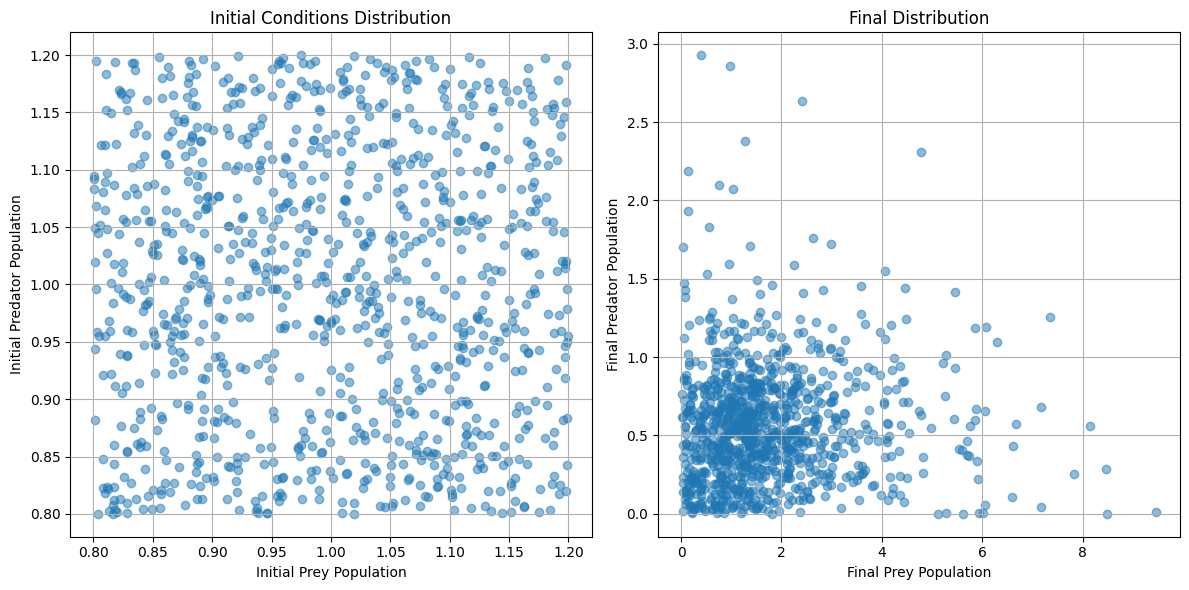
\includegraphics[width=0.8\textwidth]{initial_final_distribution}
    \caption{\textbf{Initial vs Final Distribution}. Comparison between initial conditions (left) and final states (right) of the predator-prey systems after simulation.}
    \label{fig:initial}
\end{figure}

A critical insight into the system's sensitivity to initial conditions is provided by Figure \ref{fig:initial}, which compares the initial and final states of the simulations. Despite starting from a tightly constrained parameter space (prey and predator populations both between 0.8-1.2 units), the final states display remarkable divergence. This sensitivity is a hallmark of nonlinear dynamical systems, where small differences in initial conditions can lead to vastly different outcomes over time. The final distribution shows a concentration of points at lower predator values (0.1-1.0) with prey populations spread across a much wider range (0-8), indicating that many trajectories evolve toward states where prey populations are less constrained by predator influence. This divergence from similar starting points underscores the challenge in long-term forecasting of such systems, as minor variations in inputs can amplify into major differences in outcomes.

For the current study with our limited dataset of 1,000 trajectories, we implemented a simple random split into training (70\%), validation (15\%), and testing (15\%) sets. Given the time constraints and dataset size, this approach provided a practical balance between model training and evaluation needs. However, the observed dynamics suggest several potential improvements for future work with larger datasets.

\subsubsection*{Future Improvements for Data Handling}
The observed sensitivity to initial conditions and the diverse range of dynamic behaviors have important implications for more sophisticated approaches to training, validation, and testing splits in future work. With a larger dataset, a stratified sampling approach based on the four identified clusters would better maintain the distribution of dynamic behaviors across all splits.

Such stratification would be particularly valuable because the complexity and diversity of the dynamics require the model to learn from examples across all behavioral regimes. For example, the rare "predator collapse" trajectories (1.2\% of cases) should be proportionally represented in all splits to prevent the model from treating such cases as anomalies during evaluation. Similarly, the phase relationships and oscillation characteristics vary systematically across clusters, making it essential that the model train on and be evaluated against the full spectrum of possible dynamics.


\subsubsection*{Forecasting Challenge}

The Lotka-Volterra system presents an ideal test case for evaluating language model forecasting capabilities due to its nonlinear dynamics that challenge simple forecasting methods, its requirement for simultaneous prediction of interdependent variables, the importance of long-range historical patterns for accurate prediction, its inherent periodicity that aligns with language models' pattern recognition strengths, and its well-understood mathematical properties that provide a strong basis for evaluation. Our forecasting task requires the model to predict future values $(x_{t+1}...t+n, y_{t+1}...t+n)$ given past values $(x_{t-m}...t, y_{t-m}...t)$, effectively testing the model's ability to identify and extrapolate complex numerical patterns.

\subsection*{LLMTIME Preprocessing Approach}

\subsection*{FLOPs Calculation}

\section*{Implementation}
\subsection*{Hardware}
\subsection*{Data preprocessing implementation}
\begin{itemize}
    \item Tokenization approach
    \item Numeric to text conversion details
    \item Scaling and precision considerations
\end{itemize}
\subsection*{LoRA implementation details}
include hardware
\begin{itemize}
    \item Target modules selection (Q and V projections)
    \item LoRA hyperparameters
\end{itemize}
\subsection*{Model training setup}
\begin{itemize}
    \item Optimization approach
    \item Learning rate and batch size considerations
    \item FLOP tracking
\end{itemize}

\section*{Baseline Evaluation}
\begin{itemize}
    \item Untrained model performance analysis
    \item Tokenization examples and results
    \item FLOP accounting for the Qwen2.5 model operations
    \item Analysis of accuracy metrics (MSE, MAE) for the baseline
\end{itemize}


\section*{LoRA Experiments}
\subsection*{Hyperparameter search experiment}
\subsection*{Analysis of results}

\section*{ Final Model Performance}

\begin{itemize}
    \item Detailed analysis of the best model configuration
   \item  Comparative evaluation against baseline
   \item  Visualization of forecasting performance
   \item Error analysis for prey and predator populations
\end{itemize}

\section*{ Discussion}
\begin{itemize}
    \item Analysis of the trade-offs between computational cost and accuracy
\item Impact of different hyperparameters on performance
\item Strengths and limitations of the approach
\item Recommendations for time-series fine-tuning under tight compute budgets
\end{itemize}


\section*{Conclusion}

\begin{itemize}
    \item  Summary of key findings
     \item Suggestions for future improvements
     \item Final FLOP accounting table
\end{itemize}

\section*{Appendix}
\subsection*{Detailed Flop Calculation} 

\bibliographystyle{plain}
\bibliography{references}
\end{document}